\scanpage{97}

On conclut de (7) que $\ell^N$ est \uline{complet}. Il suffit de prouver que \deleted{\unsure{toute}} \unsure{\deleted{suite}|suite} $(x^k)$ \deleted{dans $\ell^N$} d'éléments $x^k\in\ell^N$, telle que $\sum\lVert x^{k}\rVert_N<+\infty$, est sommable dans $\ell^N$. Or \deleted{elle} on aura \unsure{à|:} fortiori $\sum\lVert x^k\rVert_\infty<+\infty$, donc la \deleted{série} suite sera sommable dans $\ell^\infty$, \inserted{vers un $x\in\ell^\infty$} d'autre part on \deleted{\unsure{aura|aussi}} voit sur (7) que $x\in\ell^N$. D'autre part,

{\reversemarginpar\margin{Inutile, il suffit de procéder par dualité : $\ell^N$ est le dual de $\ell_N$.}}

on a

\[
N\left(x-\sum_{k=1}^n x^k\right)=\deleted{\unsure{\leq|\Rightarrow}}N\left(\deleted{\unsure{x-|x}}\sum_{n+1}^\infty x^k\right)\leq\sum_{n\unsure{-|+}1}^{\unsure{n|\infty}}N(x^k),
\]

qui tend vers \deleted{\unsure{l'$\infty$|zéro} \unsure{puisque la|pour}}\inserted{$0$ pour $n\to+\infty$}, puisque $\sum N(x^k)$ est une série convergente. Il s'ensuit que l'on a aussi $\sum x^k=x$ \uline{dans $\ell^N$}.

Soit $\ell_N$ l'adhérence de $C^{(\underline N)}$ dans $\ell^N$, comme $\ell^N$ est complet, $\ell_N$ s'identifie au complété de $C^{(\underline N)}$ pour la norme $N$. Il est encore trivial que si $N'\leq N''$, alors $\ell_{N'}\subset\ell_{N''}$, et \unsure{l'injection|l'application} identique $\ell_{N'}\to\ell_{N''}$ est de norme $\leq 1$. En particulier, les espaces $\ell_N$ associés à $N_1$ et $N_\infty$ étant resp. $\ell^1$ et $c_0$, on obtient

\[
\begin{array}{@{}l@{\qquad}l@{}}
(8)&\displaystyle \ell^1\subset\ell_N\subset c_0
\end{array}
\]

{\reversemarginpar\margin{
\begin{tikzpicture}[x=0.13mm,y=-0.13mm,line cap=round,line join=round]
\draw[blue!60!black,line width=0.35mm] (12,25)--(25,27)--(37,28)--(54,28)--(69,29)--(81,31)--(94,31);
\draw[blue!60!black,line width=0.3mm] (32,28)--(48,27)--(64,28)--(78,26);
\draw[blue!60!black,line width=0.3mm] (32,31)--(45,30)--(60,31)--(74,31)--(87,32);
\end{tikzpicture}}}

\uline{Proposition} On a $\ell^N\subset c_0$ sauf si $N$ est équivalente \unsure{à|:} $N_\infty$.

\deleted{Notons la formule, qui précise la \unsure{condition|propriétés} \unsure{ci-dessus|suivantes}}

\[
\begin{array}{@{}l@{\qquad}l@{}}
\deleted{(9)}&\displaystyle \deleted{\underline{\ell}_N=\underline{\ell}^N\cap\underline{c}_0}
\end{array}
\]

\deleted{Il suffit de prouver que $x\in\ell^N\cap c_0$ implique $x\in\ell_N$. \unsure{Et} En effet, on aura}\raisebox{-0.8ex}[0pt][0pt]{\makebox[0pt][r]{\begin{tikzpicture}[x=0.15cm,y=0.15cm,baseline]
\draw[line width=0.45pt] (0,0)--(0.6,0);
\fill (1.3,0) circle (0.06);
\fill (2.3,-0.02) circle (0.07);
\draw[line width=0.45pt] (3.15,-0.02)--(3.75,-0.02);
\fill (4.2,-0.02) circle (0.07);
\draw[line width=0.45pt] (5.1,-0.02)--(5.8,-0.04);
\draw[line width=0.45pt] (6.75,-0.08)--(7.65,-0.08);
\fill (8.65,-0.1) circle (0.07);
\draw[line width=0.45pt] (9.6,-0.08)--(10.2,-0.08);
\end{tikzpicture}}}

Notons que $R^{(N)}$ est en dualité avec lui-$=$ par l'accouplement $\langle x,y\rangle=\sum x_i y_i$. Cela permet de faire correspondre à \deleted{toute} une norme $N$ sur $R^{(N)}$, la \uline{norme polaire}, notée $N'$, définie par

\[
\begin{array}{@{}l@{\qquad}l@{}}
(9)&\displaystyle N^\circ(y')=\underset{N(\unsure{y|x})\leq 1}{\operatorname{Sup}}\,|\langle x,y'\rangle|
\end{array}
\]

{\reversemarginpar\margin{De plus, \unsure{alors|clairement} \unsure{on a} $(N^\circ)^\circ=N$, on peut le vérifier .... \deleted{\unsure{on est ramené} \unsure{à|au|de} \illegible{1}}}}

Si $N$ est une norme de Schatten, on vérifie
{\reversemarginpar\margin{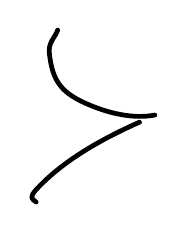
\begin{tikzpicture}[x=0.13mm,y=-0.13mm,line cap=round,line join=round]
\draw[line width=0.6mm] (45,21) .. controls (43,28) and (35,33) .. (37,45) .. controls (40,69) and (47,81) .. (71,92) .. controls (95,103) and (120,108) .. (140,104);
\draw[line width=0.6mm] (125,111) .. controls (91,126) and (50,148) .. (23,178) .. controls (18,184) and (19,186) .. (24,189);
\end{tikzpicture}}}
trivialement que $N^\circ$ est une norme de Schatten, et On \unsure{dira|dit} que \deleted{le dual de $\ell_N$ s'identifie à $\ell^{N'}$, l'accou\unsure{p|pl} \unsure{étant|ment} $\sum x_i x_i'$ est \unsure{abs\textsuperscript{t}} sommable, et que} \inserted{si $u\in\ell_N$, $u'\in\ell^{N^\circ}$, alors \deleted{\unsure{on a le}}}

{\reversemarginpar\margin{98}}

